\documentclass[tikz,border=10pt]{standalone}

\usepackage{amsmath,amssymb}
\usepackage{helvet}
\renewcommand{\familydefault}{\sfdefault}

\usetikzlibrary{arrows.meta,calc,fit,positioning,backgrounds,shadows.blur,decorations.pathmorphing}

% --- MODERN PALETTE ------------------------------------------------
\definecolor{evc}{RGB}{33, 150, 243}
\definecolor{splitc}{RGB}{0, 191, 165}
\definecolor{rawc}{RGB}{255, 145, 0}
\definecolor{truec}{RGB}{41, 45, 50}

% Reservoir colors
\definecolor{qnodeblue}{RGB}{92, 107, 192}
\definecolor{qnoderred}{RGB}{236, 64, 122}
\definecolor{qnodebg}{RGB}{248, 249, 250}
\definecolor{haloc}{RGB}{180, 195, 180}

% Accent
\definecolor{accentpink}{RGB}{255, 64, 129}

\definecolor{axisgray}{HTML}{9AA0A6}
\definecolor{muted}{HTML}{71767C}
\definecolor{edgegray}{HTML}{A7A9AC}
\definecolor{measuregray}{HTML}{737B84}
\definecolor{reservoirblue}{HTML}{3437A8}
\definecolor{reservoirred}{HTML}{B52F37}
\colorlet{accent}{reservoirred}

\tikzset{
  route/.style={
    line width=1.35pt,
    line cap=round,
    opacity=0.42,
    smooth
  },
  stagelabel/.style={
    font=\bfseries\fontsize{10.8}{11.8}\selectfont,
    text=truec
  },
  respanel/.style={
    draw=qnodeblue!15,
    fill=qnodebg,
    rounded corners=10pt,
    blur shadow={
      shadow blur steps=6,
      shadow xshift=0pt,
      shadow yshift=-2pt,
      shadow opacity=10
    }
  },
  methodbox/.style={
    rounded corners=6pt,
    fill=white,
    minimum width=3.10cm,
    minimum height=1.18cm,
    align=center,
    inner sep=3.5pt,
    blur shadow={
      shadow blur steps=4,
      shadow yshift=-1.5pt,
      shadow opacity=20
    }
  },
  qnodeB/.style={
    circle,
    shading=ball,
    ball color=qnodeblue!85!white,
    minimum size=3.0mm,
    inner sep=0pt
  },
  qnodeR/.style={
    circle,
    shading=ball,
    ball color=qnoderred!95!white,
    minimum size=3.0mm,
    inner sep=0pt
  },
  halo/.style={
    circle,
    draw=haloc,
    densely dashed,
    minimum size=4.8mm,
    inner sep=0pt,
    fill=haloc!15,
    opacity=0.6
  },
  straightedge/.style={
    draw=black!15,
    line width=0.6pt
  },
  wavyblue/.style={
    draw=qnodeblue!60,
    line width=0.75pt,
    decorate,
    decoration={snake, amplitude=0.3mm, segment length=2.2mm}
  },
  wavypink/.style={
    draw=accentpink!60,
    line width=0.75pt,
    decorate,
    decoration={snake, amplitude=0.3mm, segment length=2.2mm}
  }
}

\tikzset{
  stage/.style={font=\bfseries\fontsize{10.8}{11.6}\selectfont,text=truec},
  qblue/.style={circle,shade,ball color=reservoirblue,
                draw=reservoirblue!85!black,line width=0.35pt,
                inner sep=0pt,minimum size=11.5pt},
  qred/.style={circle,shade,ball color=reservoirred,
               draw=reservoirred!85!black,line width=0.35pt,
               inner sep=0pt,minimum size=11.5pt},
  graphlink/.style={draw=edgegray,line width=0.52pt,line cap=round},
  blueflow/.style={-{Stealth[length=3.2pt,width=2.6pt]},draw=reservoirblue,
                   line width=0.72pt,line cap=round},
  redflow/.style={-{Stealth[length=3.2pt,width=2.6pt]},draw=reservoirred,
                  line width=0.72pt,line cap=round},
}

\begin{document}
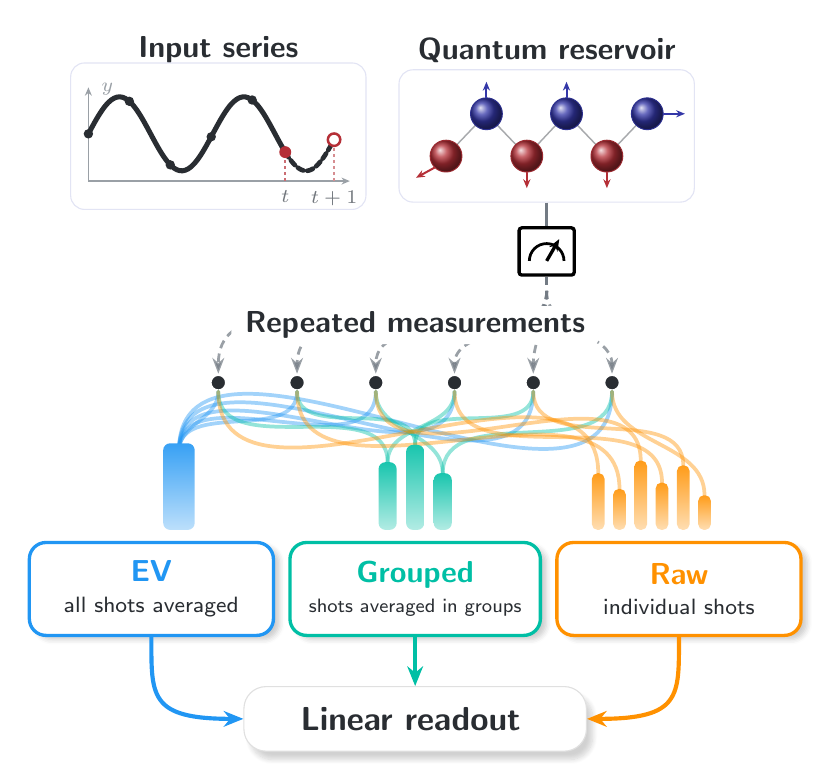
\begin{tikzpicture}[x=1cm,y=1cm]

% Shared horizontal alignment
\coordinate (EVc)    at (2.00,-4.75);
\coordinate (Splitc) at (5.35,-4.75);
\coordinate (Rawc)   at (8.70,-4.75);

% ========================================================================
% Input series: a smooth, irregular Mackey--Glass-like trace with a restrained
% forecast window.  It is deliberately not connected to the reservoir by an
% arrow: spatial alignment already communicates the processing order.
% ========================================================================
  \begin{scope}[shift={(0.70,0)}]
  \node[stage] at (2.15,2.09) {Input series};
  \node[draw=qnodeblue!18,fill=white,rounded corners=5pt,
        minimum width=3.75cm,minimum height=1.86cm] at (2.15,1.00) {};
  \def\xstart{0.50}\def\xt{3.00}\def\xtp{3.62}\def\xend{3.82}

  \draw[-{Stealth[length=3.0pt,width=2.5pt]},axisgray,line width=0.55pt]
    (\xstart,0.43) -- (\xend,0.43);
  \draw[-{Stealth[length=3.0pt,width=2.5pt]},axisgray,line width=0.55pt]
    (\xstart,0.43) -- (\xstart,1.62);
  \node[font=\scriptsize,text=axisgray,anchor=north west] at
    ($(\xstart,1.62)+(0.04,0.18)$) {$y$};

  % Both segments evaluate the same analytic sinusoid.  Splitting the path at
  % t changes only the line style, so the forecast has no artificial corner.
  \draw[truec,line width=1.82pt,line cap=round]
    plot[domain=\xstart:\xt,samples=70,smooth]
      (\x,{1.03 + 0.47*sin(360*(\x-0.50)/1.58)});
  \draw[truec,line width=1.68pt,dash pattern=on 2.2pt off 1.45pt,
        line cap=round]
    plot[domain=\xt:\xtp,samples=28,smooth]
      (\x,{1.03 + 0.47*sin(360*(\x-0.50)/1.58)});

  % Sparse samples make the finite observed record explicit without clutter.
  \foreach \sx in {0.50,1.02,1.54,2.06,2.58}{
    \fill[truec] (\sx,{1.03 + 0.47*sin(360*(\sx-0.50)/1.58)}) circle (1.70pt);
  }

  \coordinate (tmark) at (\xt,{1.03 + 0.47*sin(360*(\xt-0.50)/1.58)});
  \coordinate (tpone) at (\xtp,{1.03 + 0.47*sin(360*(\xtp-0.50)/1.58)});
  \draw[accent!70,line width=0.65pt,dash pattern=on 1pt off 1.2pt]
    (\xt,0.43) -- (tmark);
  \draw[accent!55,line width=0.65pt,dash pattern=on 1pt off 1.2pt]
    (\xtp,0.43) -- (tpone);
  \fill[accent] (tmark) circle (2.15pt);
  \draw[accent,line width=0.90pt,fill=white] (tpone) circle (2.25pt);
  \node[font=\scriptsize,text=muted,anchor=north] at (\xt,0.43) {$t$};
  \node[font=\scriptsize,text=muted,anchor=north] at (\xtp,0.43) {$t+1$};
  \end{scope}

% ========================================================================
% Frozen six-qubit line reservoir.  The six nodes and five links match the
% actual hardware circuit; alternating colors indicate heterogeneous local
% rotations, not two different qubit species.
% ========================================================================
  \begin{scope}[shift={(7.02,0.76)},x=0.90cm,y=0.64cm]
    \node[stage] at (0,2.08) {Quantum reservoir};

    % A restrained module boundary separates the quantum circuit from the
    % surrounding page without competing with the colored method boxes.
    \node[draw=qnodeblue!18,fill=white,rounded corners=5pt,
          minimum width=3.75cm,minimum height=1.68cm] (reservoirpanel) at (0,0.38) {};

    \coordinate (cq0) at (-1.42,-0.02);
    \coordinate (cq1) at (-0.85,0.82);
    \coordinate (cq2) at (-0.28,-0.02);
    \coordinate (cq3) at ( 0.28,0.82);
    \coordinate (cq4) at ( 0.85,-0.02);
    \coordinate (cq5) at ( 1.42,0.82);

    \foreach \a/\b in {cq0/cq1,cq1/cq2,cq2/cq3,cq3/cq4,cq4/cq5}{
      \draw[graphlink] (\a) -- (\b);
    }

    \node[qred]  (r1) at (cq0) {};
    \node[qblue] (b1) at (cq1) {};
    \node[qred]  (r2) at (cq2) {};
    \node[qblue] (b2) at (cq3) {};
    \node[qred]  (r3) at (cq4) {};
    \node[qblue] (b3) at (cq5) {};
    % Anchor preserves the meter geometry independently of the visible panel.
    \node[fit=(r1)(b1)(r2)(b2)(r3)(b3),
          inner sep=1.5pt] (resbox) {};

    \draw[redflow]  (r1.south west) -- ++(-0.26,-0.20);
    \draw[blueflow] (b1.north) -- ++(0,0.31);
    \draw[redflow]  (r2.south) -- ++(0,-0.31);
    \draw[blueflow] (b2.north) -- ++(0,0.31);
    \draw[redflow]  (r3.south) -- ++(0,-0.31);
    \draw[blueflow] (b3.east) -- ++(0.30,0.00);
    \coordinate (reservoirout) at (0.00,-0.82);
  \end{scope}

% ===================================================================
% (3) REPEATED MEASUREMENTS
% ===================================================================
\foreach \i/\x in {1/2.85,2/3.85,3/4.85,4/5.85,5/6.85,6/7.85}{
  \node[circle, fill=truec, draw=white, line width=0.8pt, inner sep=2pt] (s\i) at (\x,-2.13) {};
}

\coordinate (mPos) at ($(reservoirpanel.south)+(0.00,-0.62)$);
\node[draw=black, fill=white, minimum width=0.7cm, minimum height=0.6cm, line width=1.2pt, rounded corners=1pt] (meas) at (mPos) {};
\coordinate (mBase) at ($(meas.center)+(0,-0.12)$);
\draw[black, line width=1pt] ($(mBase)+(-0.22,0)$) arc[start angle=180, end angle=0, radius=0.22];
\draw[-{Stealth[length=1.5mm, width=1.2mm]}, black, line width=1.2pt] (mBase) -- ++(60:0.32);

\draw[measuregray, line width=1.05pt]
  (reservoirpanel.south) -- (meas.north);
\coordinate (mstemBot) at ($(meas.south)+(0.00,-0.18)$);
\draw[measuregray, line width=1.05pt, densely dashed] (meas.south) -- (mstemBot);

\foreach \i/\target in {1/s1,2/s2,3/s3,4/s4,5/s5,6/s6}{
  \draw[-{Stealth[length=2mm, width=1.5mm]}, measuregray,
        line width=1.0pt, densely dashed, opacity=0.72]
        (mstemBot) to[out=-90, in=90] (\target);
}

\node[stagelabel, anchor=center, fill=white, rounded corners=2pt, inner xsep=5pt, inner ysep=2pt] at (5.35,-1.40) {Repeated measurements};

% ===================================================================
% (4) WATERFALL ROUTES + BARS
% ===================================================================
\coordinate (EVbaseSW) at (2.15,-4.00);
\coordinate (EVbaseNE) at (2.55,-2.90);
\coordinate (EVjoin)   at (2.35,-3.00);

\coordinate (SplitA) at (5.00,-3.14);
\coordinate (SplitB) at (5.35,-2.92);
\coordinate (SplitC) at (5.70,-3.28);

\foreach \name/\x/\h in {rawA/7.675/0.72, rawB/7.945/0.52, rawC/8.215/0.88, rawD/8.485/0.60, rawE/8.755/0.82, rawF/9.025/0.44}{
  \coordinate (\name) at (\x,{ -4.00 + \h });
}

\foreach \i in {1,...,6}{
  \draw[evc, route] (s\i) to[out=-90, in=90] (EVjoin);
}
\foreach \i/\target in {1/SplitA,2/SplitB,3/SplitC,4/SplitA,5/SplitB,6/SplitC}{
  \draw[splitc, route] (s\i) to[out=-90, in=90] (\target);
}
\foreach \i/\target in {1/rawA,2/rawB,3/rawC,4/rawD,5/rawE,6/rawF}{
  \draw[rawc, route] (s\i) to[out=-90, in=90] (\target);
}

\path[top color=evc!90, bottom color=evc!30, rounded corners=2.5pt] (EVbaseSW) rectangle (EVbaseNE);
\foreach \x/\h in {4.885/0.86,5.235/1.08,5.585/0.72}{
  \path[top color=splitc!90, bottom color=splitc!30, rounded corners=2.5pt] (\x,-4.00) rectangle ++(0.23,\h);
}
\foreach \x/\h in {7.595/0.72,7.865/0.52,8.135/0.88,8.405/0.60,8.675/0.82,8.945/0.44}{
  \path[top color=rawc!90, bottom color=rawc!30, rounded corners=2pt] (\x,-4.00) rectangle ++(0.16,\h);
}

% ===================================================================
% (5) METHOD BOXES -- simple labels only
% ===================================================================
\node[methodbox, draw=evc, line width=1.2pt] (EVlab) at (EVc) {%
  {\bfseries\fontsize{10.5}{11}\selectfont\color{evc}EV}\\[-0.2ex]
  {\fontsize{7.8}{8.4}\selectfont\color{truec}all shots averaged}
};

\node[
  methodbox,
  draw=splitc,
  line width=1.2pt,
  minimum width=3.18cm
] (Splitlab) at (Splitc) {%
  {\bfseries\fontsize{10.5}{11}\selectfont\color{splitc}Grouped}\\[-0.2ex]
  {\fontsize{6.7}{7.4}\selectfont\color{truec}shots averaged in groups}
};

\node[methodbox, draw=rawc, line width=1.2pt] (Rawlab) at (Rawc) {%
  {\bfseries\fontsize{10.5}{11}\selectfont\color{rawc}Raw}\\[-0.2ex]
  {\fontsize{7.6}{8.3}\selectfont\color{truec}individual shots}
};

% ===================================================================
% (6) LINEAR READOUT
% ===================================================================
\node[
  draw=black!12,
  fill=white,
  rounded corners=8pt,
  minimum width=4.35cm,
  minimum height=0.82cm,
  align=center,
  blur shadow={shadow blur steps=8, shadow yshift=-3pt, shadow opacity=18}
] (readout) at (5.35,-6.40) {%
  {\bfseries\fontsize{12.5}{13}\selectfont\color{truec}Linear readout}
};

\draw[-{Stealth[length=2.5mm, width=2mm]}, evc, line width=1.5pt]
  (EVlab.south) .. controls +(0,-0.75) and +(-1.2,0) .. (readout.west);

\draw[-{Stealth[length=2.5mm, width=2mm]}, splitc, line width=1.5pt]
  (Splitlab.south) .. controls +(0,-0.55) and +(0,0.8) .. (readout.north);

\draw[-{Stealth[length=2.5mm, width=2mm]}, rawc, line width=1.5pt]
  (Rawlab.south) .. controls +(0,-0.75) and +(1.2,0) .. (readout.east);

\end{tikzpicture}
\end{document}
